%%---------------------------------------------------------------------------%%
%% report.tex
%% Tom Evans
%% Wednesday January 4 13:31:55 2017
%% Copyright (C) 2008-2017 Oak Ridge National Laboratory, UT-Battelle, LLC.
%%---------------------------------------------------------------------------%%

% Add the 'draft' option to compile faster (without images e.g.)
%\documentclass[draft]{ecpreport}
\documentclass{ecpreportv2}
\usepackage[binary-units,per-mode=symbol-or-fraction]{siunitx}
\usepackage{multirow}
\usepackage{float}
\usepackage[shortcuts]{glossaries}
\usepackage{algorithm}          % Provides algorithm environment
\usepackage{algorithmicx}       % Provides algorithmic block
\usepackage{algpseudocode}      % Option of algorithmicx package
\usepackage{caption}
\usepackage{subcaption}
\usepackage{cite}
\usepackage[nameinlink,capitalize]{cleveref}


\renewcommand{\sectionautorefname}{\S}
\renewcommand{\subsectionautorefname}{\S}
\renewcommand{\subsubsectionautorefname}{\S}
\renewcommand{\equationautorefname}{Eq.}

\newcommand{\iso}[2][]{\ensuremath{\left.^{\text{{#2}}}\text{{#1}}\right.}}

\usepackage{array}
\newcolumntype{L}[1]{>{\raggedright\let\newline\\\arraybackslash\hspace{0pt}}m{#1}}
\newcolumntype{C}[1]{>{\centering\let\newline\\\arraybackslash\hspace{0pt}}m{#1}}
\newcolumntype{R}[1]{>{\raggedleft\let\newline\\\arraybackslash\hspace{0pt}}m{#1}}
\newcolumntype{P}{S[round-mode=places,round-precision=4,
                    table-format=-1.4e-2,output-exponent-marker=\text{e}]}
\newcolumntype{Q}{S[round-mode=places,round-precision=3,
                    table-format=-1.3e-1,output-exponent-marker=\text{e}]}


\let\DeclareUSUnit\DeclareSIUnit
\let\US\SI
\DeclareUSUnit\inch{in}
\DeclareUSUnit\psia{psia}
\DeclareSIUnit\src{source}

\newcommand{\milestone}[1]{\href{https://jira.exascaleproject.org/projects/ADSE08/issues/#1}{#1}}

%%---------------------------------------------------------------------------%%
%% VARIABLES
%%---------------------------------------------------------------------------%%
\author{
  Elia Merzari, ANL, PSU
  \and Jun Fang, ANL
  \and Dillon Shaver, ANL
  \and Misun Min, ANL
  \and Paul Fischer, ANL
  \and Yu-Hsinag Lan, ANL
  \and Ronald Rahaman, ANL
  \and Paul Romano, ANL
}
\title{Initial full core SMR simulations with Nek5000 and NekRS}
\date{\today}
\wbs{XXX}
\id{XXX}
\reportnum{ECP-U-2020-XXX}

\submitter{Elia Merzari}

\concurrence{Steve Hamilton}
\concurrenceorg{Oak Ridge National Laboratory}

\concurrence{Thomas Evans}
\concurrenceorg{Oak Ridge National Laboratory}

\approver{Andrew Siegel}
\approverorg{Argonne National Laboratory}

\setacronymstyle{long-short}
\makeglossaries
% These are acronyms used with \ac{label} or \acp{label} for plural

\newacronym{anl}{ANL}{Argonne National Laboratory}
\newacronym{ansi}{ANSI}{American National Standards Institute}
\newacronym{api}{API}{application programming interface}
\newacronym{avx}{AVX}{Advanced Vector Extensions}
\newacronym{beavrs}{BEAVRS}{Benchmark for Evaluation and Validation of Reactor Simulations}
\newacronym{cfd}{CFD}{computational fluid dynamics}
\newacronym{sgmv}{SGMV}{spacer grid and mixing vanes}
\newacronym{ce}{CE}{continuous-energy}
\newacronym{cpi}{CPI}{clock cycles per instruction}
\newacronym{dmm}{DMM}{Device Memory Manager}
\newacronym{dram}{DRAM}{Dynamic random-access memory}
\newacronym{elf}{ELF}{Executable and Linkable Format}
\newacronym{fom}{FOM}{figure of merit}
\newacronym{gll}{GLL}{Gauss-Lobatto-Legendre}
\newacronym{gpu}{GPU}{graphical processing unit}
\newacronym{isa}{ISA}{instruction set architecture}
\newacronym{jlse}{JLSE}{Joint Laboratory for System Evaluation}
\newacronym{kpp}{KPP}{Key Performance Parameter}
\newacronym{knc}{KNC}{Knights Corner}
\newacronym{knl}{KNL}{Knights Landing}
\newacronym{lwr}{LWR}{light water reactor}
\newacronym{mc}{MC}{Monte Carlo}
\newacronym{mcdram}{MCDRAM}{Multi-Channel DRAM}
\newacronym{mlbw}{MLBW}{multilevel Breit-Wigner}
\newacronym{mpi}{MPI}{Message Passing Interface}
\newacronym{nrc}{NRC}{Nuclear Regulatory Commission}
\newacronym{numa}{NUMA}{non-uniform memory access}
\newacronym{ornl}{ORNL}{Oak Ridge National Laboratory}
\newacronym{olcf}{OLCF}{Oak Ridge Leadership Computing Facility}
\newacronym{phi}{PHI}{Xeon Phi}
\newacronym{pod}{POD}{plain old data}
\newacronym{pwr}{PWR}{pressurized water reactor}
\newacronym{rm}{RM}{Reich-Moore}
\newacronym{simd}{SIMD}{single instruction multiple data}
\newacronym{smr}{SMR}{small modular nuclear reactor}
\newacronym{snc}{SNC}{sub-NUMA cluster}
\newacronym{stl}{STL}{Standard Template Library}
\newacronym{tdp}{TDP}{thermal design power}
\newacronym{vf}{VF}{vector fitting}
\newacronym{vpu}{VPU}{vector processing unit}
\newacronym{wmp}{WMP}{windowed multipole}


% US units
\let\DeclareUSUnit\DeclareSIUnit
\let\US\SI
\DeclareUSUnit\inch{in}

%%---------------------------------------------------------------------------%%
%% FRONT MATTER
%%---------------------------------------------------------------------------%%

\begin{document}
\frontmatter

%%---------------------------------------------------------------------------%%
%% REVISION LOG

\begin{revlog}
  1.0 & \today & Original & \\\hline
\end{revlog}

%%---------------------------------------------------------------------------%%
% EXECUTIVE SUMMARY

\begin{abstract}

This document describes the completion of ExaSMR milestone ``Full core simulations'' (JIRA ID \milestone{ADSEXX}).  As part of this milestone for the first time, a novel set of pin-resolved computational fluid dynamics (\ac{cfd}) full-core simulations have been performed. These simulations represent a significant increase in capability in what is now possible with \ac{cfd} on pre-Exascale systems. The simulations have been performed with the spectral element solvers NekRS on the supercomputer Summit. Multiple simulations campaigns have been conducted: (1) LES simulations in bare bundle, (2) RANS simulations in bare bundles, (3) RANS simulations with momentum sources and (4) Conjugate heat transfer calculations.

\end{abstract}

\tableofcontents
\listoffigures
\listoftables
\newpage
\printglossary

%%---------------------------------------------------------------------------%%
% MAIN DOCUMENT
%%---------------------------------------------------------------------------%%

\mainmatter
\section{Introduction}

The ExaSMR project is developing tools for coupling \acf{mc} radiation
transport solvers to a \acf{cfd} solver.  Work is based on the Shift MC, OpenMC MC, and Nek5000/NekRS CFD codes. The application development objective is to optimize these applications for exascale execution of full core simulations and modularize and integrate them into a common framework for coupled and individual execution. The work is supported by secondary applications for data processing and third-party libraries.
Given the sheer scale of nuclear systems, the main algorithmic driver on the CFD side is weak scaling.
The focus for the first four years is  on demonstrating scaling up to a full reactor core for high-fidelity simulation of turbulence. The goals is to demonstrate full-core fluid calculations aimed at better predicting the steady-state performance. The first step is performing URANS calculations, then analysis will be conducted with zonal hybrid LES-RANS that provides an additional scaling dimension besides the number of assemblies. LES may be used to simulate a portion of a core, while the remainder will be handled by RANS.

A key aspect of the modeling of PWR fuel assemblies is the presence of spacer grids and the mixing promoted by mixing vanes or equivalents. In the case of fine-scale LES simulations, the grids can be modeled explicitly. In our URANS simulations we used an reduced order methodology based on momentum sources to mimic the mixing of the vanes. The momentum sources have been carefully calibrated with detailed LES simulations of spacer grids performed with Nek5000.

In previous milestones for the ExaSMR project we have focused on assembly level simulations with Nek5000 to assess baseline performance. We now shift focus to full core simulations. In fact, \textit{this milestones provides the first full-core pin resolved simulations ever performed to our knowledge}. \textbf{This represents a significant advancement in capability for the CFD of nuclear reactors}. This has been made possible by the CEED and ExaSMR investment in a novel port of Nek5000, labeled NekRS. NekRS was released in 2018 and it is developing rapidly, with significant improvements in performance. All large-scale simulations performed here have been conducted on the supercomputer Summit.

As a first step we discuss briefly the status of NekRS and some recent code improvements performed in collaboration with CEED.   Then we discuss the development of the momentum source models and the calibration procedure used. The methodology will need to be further extended and tested on more grids, but it shows a great deal of potential for the type of analysis presented here. We then discuss a series of full core analysis that have been performed as part of this study and the related numerical setups. In the results section we discuss selected outcomes of the simulation campaigns performed including some performance results. Finally an updated FOM is provided and some conclusions are discussed.

We reiterate  that the work presented here is in close collaboration with the CEED project.
%%---------------------------------------------------------------------------%%

%%---------------------------------------------------------------------------%%
\section{NekRS: recent developments enabling large scale ExaSMR simulations}
\label{sec:nekrs}

%%---------------------------------------------------------------------------%%
\section{Development of the Momentum Source Model}
\label{sec:msm}

\subsection{Overview}
\label{sec:msm1}

The CFD calculations in ExaSMR are carried out by the state-of-the-art flow solver, Nek5000/NekRS.
Though Nek5000 is able to simulate flow in complex engineering geometries, such as \acf{sgmv} \cite{BUSCO2019144}, the objective here is to model the effect of SGMV on fluid flow without a need of body-fitted mesh.
This approach would significantly reduce the number of elements (i.e., degrees of freedom) required for domain discretization and the per-subchannel computational cost. In doing so, one can greatly expand the computational domain size (up to the full core) and study the system behavior concerning the neutronics and thermal-hydraulics.
Since the Reynolds number expected in the reactor core is high, it is necessary to use a RANS approach to model turbulence as the computational expense associated with resolving the turbulent fluctuations using LES/DNS approach would be prohibitively huge.
A newly implemented $k-\tau$ RANS model is adopted in the related Nek5000 calculations.
There have been several studies in the literature reporting various attempts to explore \ac{sgmv} modeling for either CFD or subchannel analysis.
Capone et al. (2016) developed a framework to force local flow fields (in RANS simulations) to match higher-fidelity numerical solutions (e.g. LES) where the \ac{sgmv} is explicitly resolved~\cite{Capone2016}.
Mikuž and Roelofs later proposed a porosity model for the mixing grid that can be used in CFD analysis with very coarse grids~\cite{Mikuz2020}.
Meanwhile, Mao et al. (2017) developed a distributed resistance method (DRM) to model the mixing vane crossflow in subchannel analysis~\cite{Mao2017}.
However, none of the aforementioned approaches is well suited for the current investigation where both the solution accuracy and parallel computing efficiency are demanded.
Specifically, the modeling of SGMV effect here is achieved by implementing novel 3-D momentum sources to reproduce the macroscopic impact of SGMV on the coolant flow, including the magnitudes of flow swirling, inter-subchannel mixing as well as the pressure loss.
The validity of this reduced-order modeling approach is further assessed by comparing the corresponding results with those from reference LES calculations for a 5x5 pin bundle geometry with the spacer grid and mixing vanes explicitly represented.
The current work is a crucial stepping stone to fully leverage the supercomputing and cutting-edge CFD techniques in addressing grand challenges in nuclear engineering.


\subsection{Momentum Source Model Setup}
\label{sec:msm2}

The nuclear fuel rods are generally arranged together in a triangle or square pattern with supporting structures, such as the spacer grid, to hold them in place.
The mixing vanes are installed on some of the spacer grids to further promote the turbulence mixing, and thus improve the convective heat transfer from the fuel rod surface to the coolant.
The existence of the spacer grid and mixing vanes generates complex flow structures inside the core. Two major macroscopic effects are targeted in this work:
(i) the magnitude of lateral flow mixing and associated decay rate downstream of the SGMV region;
(ii) the streamwise pressure/friction loss due to the SGMV.
The flow mixing has a direct impact on the convective heat transfer performance (i.e., local Nusselt number) while the knowledge of pressure loss caused by SGMV can help better predict the required pump head to drive the coolant flow under various operating or accident conditions.
As shown in Figure~\ref{fig:sgmvcad}, a 5x5 fuel rod bundle geometry is simulated using LES with the explicit representation of detailed geometric structures including the spacer grid and mixing vanes.
Four Reynolds numbers are investigated: 10,000, 20,000, 40,000 and 80,000.
The discretization of the fuel bundle geometry results in 3.24 million spectral elements. The simulations were carried out on the IBM Blue Gene/Q Mira supercomputer at Argonne National Laboratory (ANL).
Corresponding results will be used to develop/calibrate the momentum sources in RANS calculations that would reproduce the macroscopic effects induced by the SGMV on the coolant flow.

\begin{figure}[!ht]
\centering
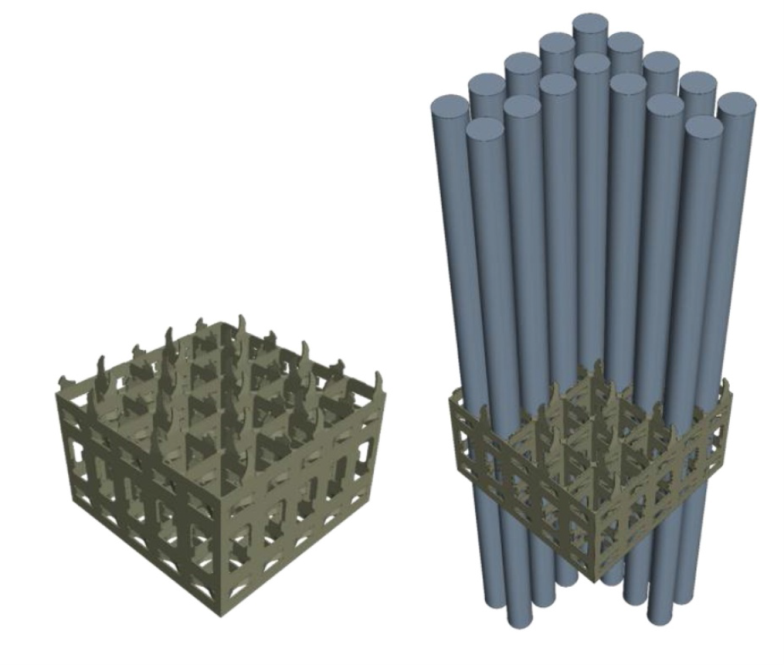
\includegraphics[width=0.5\textwidth]{./figures/3DModel_of_SGMV.png}
\caption{The structure of spacer grid and mixing vanes and a 5x5 fuel rod bundle. }
\label{fig:sgmvcad}
\end{figure}

The development of momentum sources relies on lightweight test cases with quick turnaround time. As shown in Figure~\ref{fig:model2x2}, a 2x2 bundle is created for that purpose, which is the conduit bounded by 9 neighboring fuel pins. The subchannel pitch-to-diameter ratio is 1.33, where the pitch is defined as the distance of two fuel pin centers and the pin diameter is 9.50 mm. The 2x2 bundle has a span of 10 hydraulic diameters. Inflow and outflow conditions are specified for the channel inlet and outflow. Periodic boundary condition is applied to transverse faces while no-slip wall condition applied to all fuel rod surfaces. The computational grid of 2x2 bundle case consists of 59.14 K elements (Figure~\ref{fig:model2x2}). Once the momentum sources are successfully tested in the 2x2 bundle, the next step is to extend the testing geometry to an entire assembly, and eventually to the full core.

\begin{figure}[!ht]
\centering
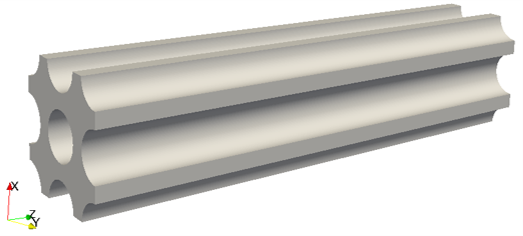
\includegraphics[width=0.5\textwidth]{./figures/3DModel_of_bundle2x2.png}
\caption{A 2x2 subchannel geometry for momentum source development and testing. }
\label{fig:model2x2}
\end{figure}

To drive the flow circulation in a subchannel which has no SGMV, the lateral momentum source terms are devised as follows
\begin{equation}
  S_x = -\frac{\eta(r)\cdot r sin(\theta)}{\tau_\text{coupling}}\\
\end{equation}

\begin{equation}
  S_y = \frac{\eta(r)\cdot r cos(\theta)}{\tau_\text{coupling}}\\
\end{equation}
where $\eta$ is a nominal angular velocity;
$r$ is the distance from any point to the reference location, that is, the subchannel centerline;
$\theta$ is the angle between the distance vector and positive x direction and
$\tau_\text{coupling}$ is the coupling time scale.
In prototypical fuel rod assembly design, the mixing vanes are deflected in different directions among neighboring subchannels (Figure~\ref{fig:sgmvcad}).
To better reflect that arrangement, each subchannel in the 2x2 bundle test is also given a major axis where the source term in the corresponding direction is enabled (as shown in Figure~\ref{fig:sblines}).
The source terms are considered as the additions to the body force term in the momentum conservation equations, which are to generate the desired flow rotation or pressure drop.
The macroscale flow movement on the cross-sectional plane is decomposed into two parts: the flow swirling within a specific subchannel and the crossflow among neighboring subchannels.
Following the examples of Chang et al. \cite{Chang2014},
a swirling factor ($F_\text{swirl}$) and a mixing factor ($F_\text{mix}$) are defined to quantify the swirling and inter-subchannel crossflow, respectively.
The absolute value of normalized velocity is averaged over the diagonal lines to obtain the swirling factor and over the gap lines to obtain the mixing factor (Figure~\ref{fig:sblines}).
\begin{equation}
  F_\text{swirl} = \frac{1}{l}\int\frac{\abs{V_\text{diag}}}{V_\text{stream}}dl\\
\end{equation}

\begin{equation}
  F_\text{mix} = \frac{1}{l}\int\frac{\abs{V_\text{gap}}}{V_\text{stream}}dl\\
\end{equation}

\begin{figure}[!ht]
\centering
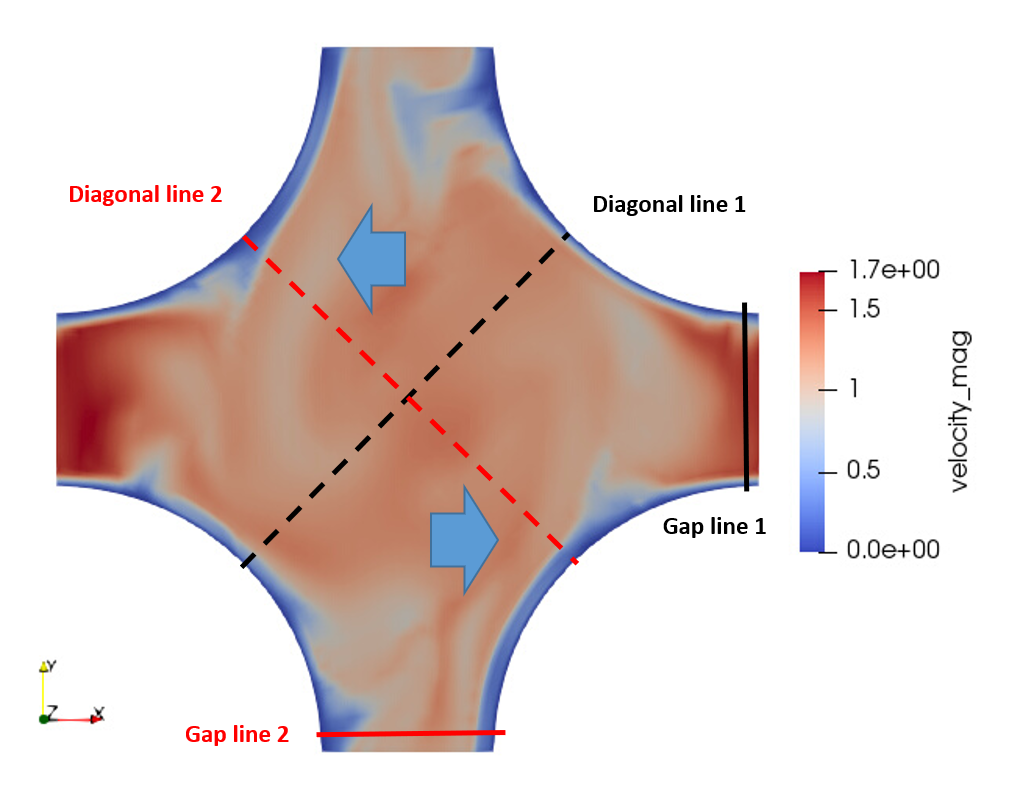
\includegraphics[width=0.5\textwidth]{./figures/Analysis_locations_in_a_subchannel.png}
\caption{The line locations to obtain swirling and mixing factors. Blue arrows indicate the deflection of the simulated mixing vanes. }
\label{fig:sblines}
\end{figure}

The streamwise pressure loss is modeled by adding a momentum source term opposite to the streamwise direction.

\begin{equation}
  S_z = -\frac{\tau_w \cdot A_\text{wet}}{V_\text{channel}}=-\frac{\tau_w \cdot A_\text{wet}}{A_\text{wet} \cdot H}=-\frac{\tau_w}{H}\\
\end{equation}

\begin{equation}
  \tau_w = C_fu^2\\
\end{equation}
where $\tau_w$ is the total shear stress caused by the SGMV structures and
$C_f$ is the effective friction coefficient;
$A_\text{wet}$ is the wetted area of channel walls;
$H$ is the height/distance over which the shear stress is exerted.
Necessary calibration is to be carried out to find out an appropriate friction coefficient that can accurately account for the pressure loss due to SGMV blockage and surface friction.


\subsection{Model Calibration and Verification}
\label{sec:msm3}

The LES of the 5x5 pin bundle were successfully performed and a substantial amount of flow information is collected.
The instantaneous velocity fields are shown in Figure~\ref{fig:velles}, from which a strong flow mixing is observed caused by the SGMV presence.
The LES cases with higher Reynolds numbers are restarted from the turbulence field fully developed at a lower Reynolds number.
In other words, the flow solutions obtained at a lower Re serve as the initial condition for the cases at higher Re, which results in significant savings in terms of computing hours.
Time-averaged first and second order flow quantities are gathered from all cases.
The subchannel highlighted with a red box is selected for further post-processing. The swirling and mixing factors as well as the pressure drop are extracted from LES flow solutions as the reference to calibrate the corresponding RANS momentum sources

\begin{figure}[!ht]
\centering
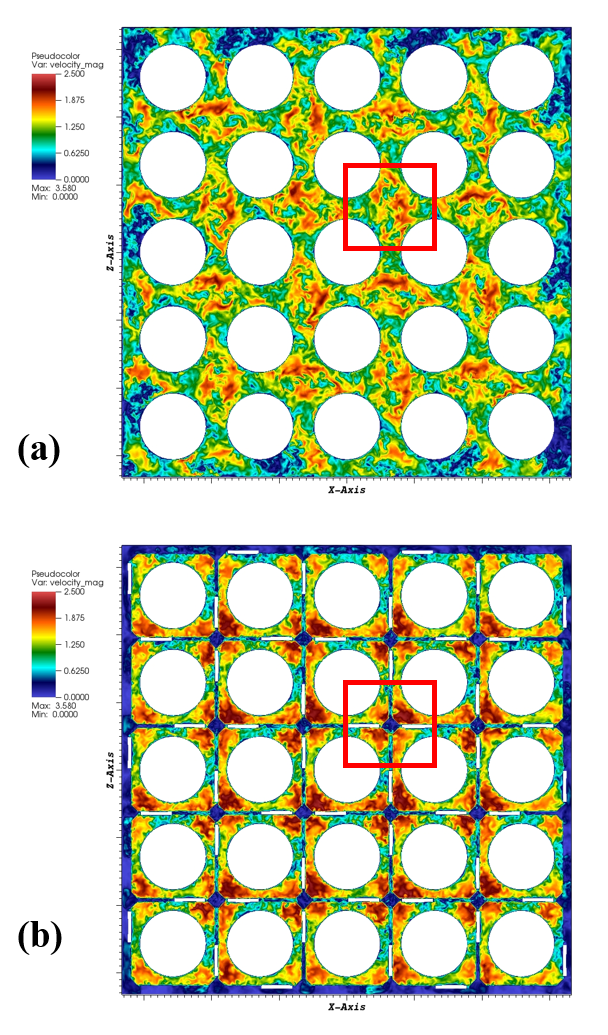
\includegraphics[width=0.5\textwidth]{./figures/LES_solutions_bundle5x5.png}
\caption{The instantaneous velocity fields at (a) a downstream location after SGMV, (b) the onset of mixing vanes region. The subchannel selected for post-processing is highlighted with a red box. }
\label{fig:velles}
\end{figure}

In the meantime, the momentum sources as introduced previously are first implemented in the 2x2 bundle test.
Interesting results are produced. Note that the test cases are RANS based and thus they would not be able to reproduce a flow field with very fine scale flow fluctuations as shown in Figure~\ref{fig:velles}.
The primary research objective here is to reproduce time-averaged macroscale flow characteristics, more specifically, the lateral/cross-sectional flow mixing and the streamwise pressure drop.
As illustrated in Figure~\ref{fig:streamline}, the momentum sources applied close to the inlet have triggered a streamline pattern shift from a parallel pattern into a swirling pattern.

\begin{figure}[!ht]
\centering
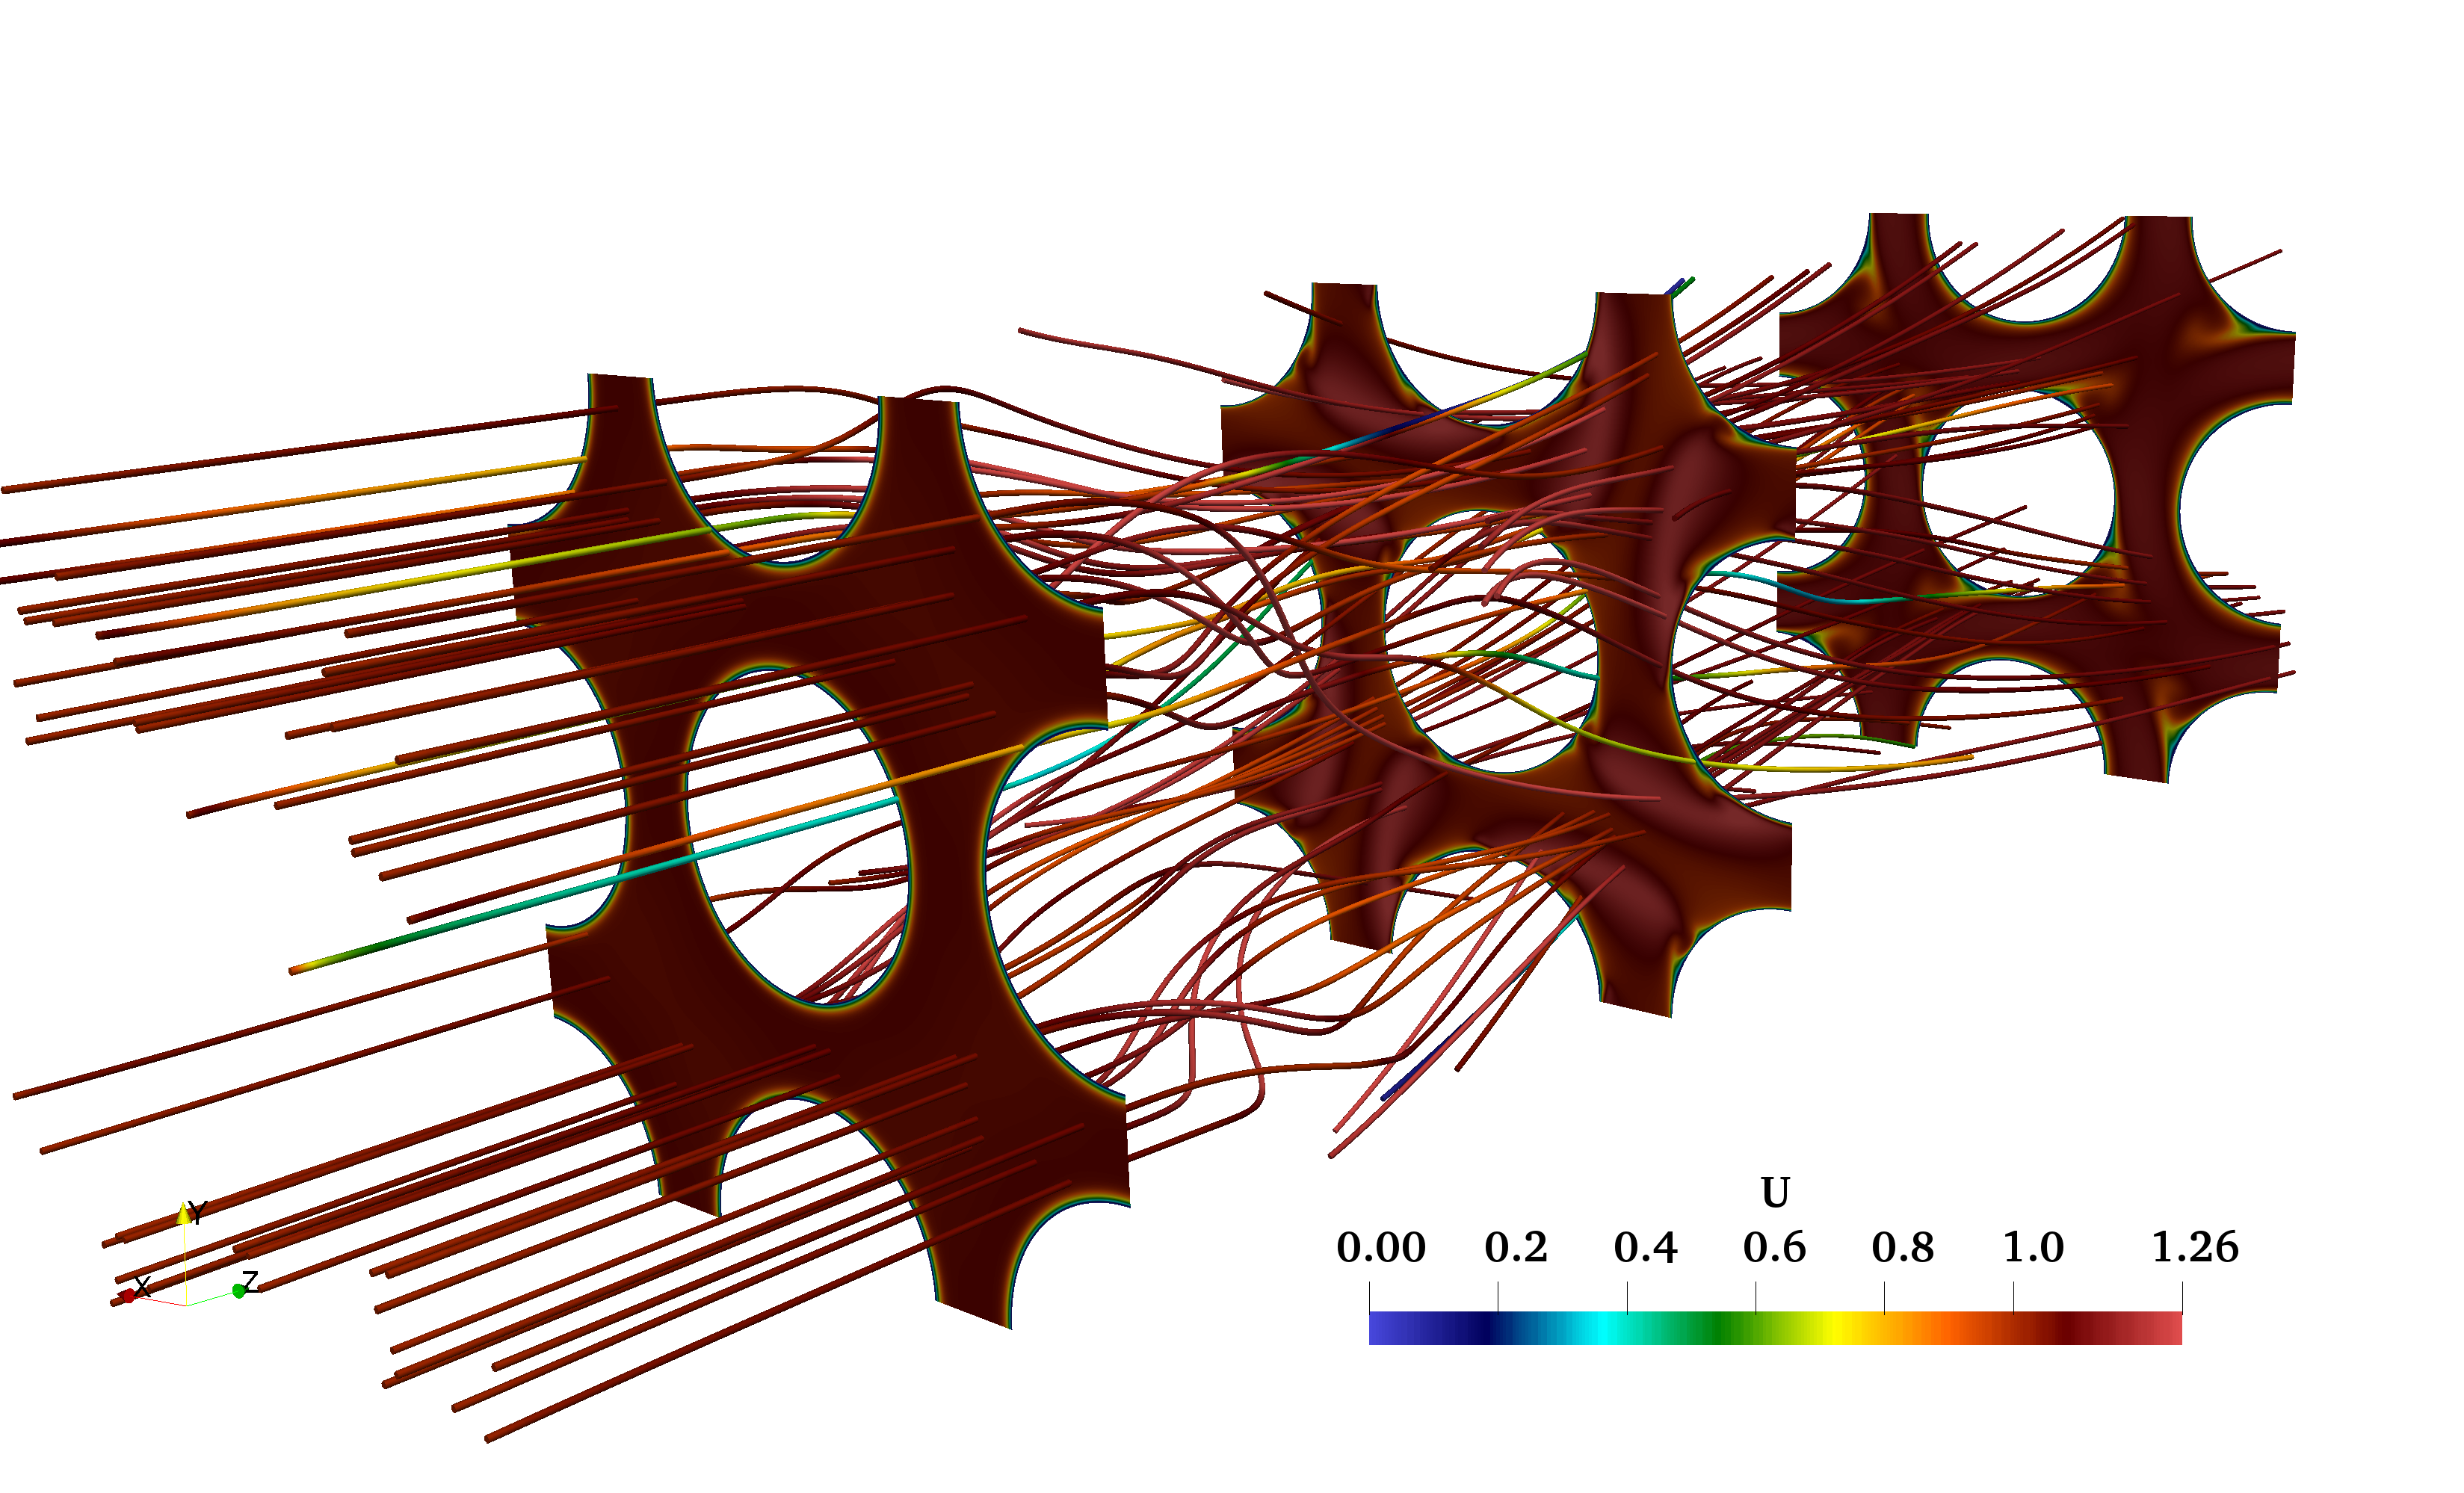
\includegraphics[width=0.5\textwidth]{./figures/RANS_streamlines_bundle2x2.png}
\caption{Streamlines revealing the flow rotation generated by the momentum sources. }
\label{fig:streamline}
\end{figure}

As the two most important figures of merit (FOM) in describing the cross-sectional flow behavior, the swirling and mixing factors are extracted from LES reference solutions.
The corresponding values serve as an anchor in the calibration of lateral momentum sources dedicated for RANS calculations.
The comparisons of swirling and mixing factor are presented in Figure~\ref{fig:fswirl} and Figure~\ref{fig:fmix}, respectively.
It is clearly demonstrated that the RANS momentum sources developed can successfully reproduce the time-averaged macroscale flow physics revealed by the high-fidelity LES reference.
The momentum sources not only produce the equivalent magnitude of flow swirling and inter-subchannel crossflow, but also capture the consistent decay trend as the flow moves further downstream from the mixing vanes.
As shown in Figure~\ref{fig:fswirl}, due to the mixing vanes deflection, the swirling factors estimated for two perpendicular diagonal lines are noticeably different, and this pattern is well represented by the lateral momentum sources.
On the other hand, the difference in mixing factors across the two gap lines is relatively smaller. Such a difference is not captured in the RANS calculation and the difference in mixing factors across two perpendicular gap lines is negligible.
Nevertheless, the RANS mixing factor results are in very good agreement with the averaged value from LES reference. For both the swirling and mixing factors, larger discrepancies are noticed right after the mixing vanes, within 2 hydraulic diameters distance, which indicates room for further improvement of current lateral momentum sources.

\begin{figure}[!ht]
\centering
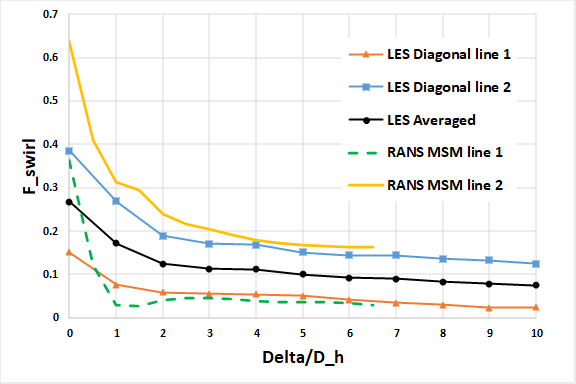
\includegraphics[width=0.5\textwidth]{./figures/Results_swirling_factor.png}
\caption{Comparison of the swirling factors from LES reference and the RANS test with momentum sources at Re = 10,000. }
\label{fig:fswirl}
\end{figure}

\begin{figure}[!ht]
\centering
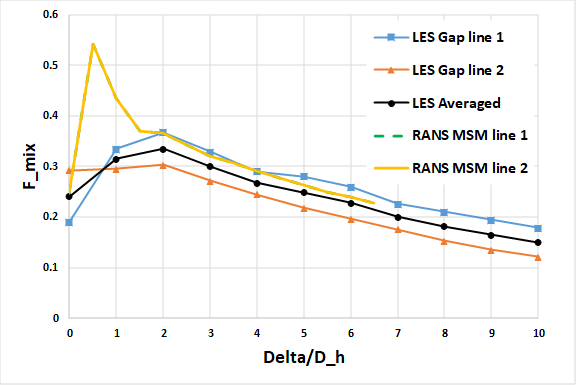
\includegraphics[width=0.5\textwidth]{./figures/Results_mixing_factor.png}
\caption{Comparison of the mixing factors from LES reference and the RANS test with momentum sources at Re = 10,000. }
\label{fig:fmix}
\end{figure}

Besides the swirling and mixing factors, the streamwise pressure loss is another key FOM to quantify the impact of spacer grid and mixing vanes on the coolant flow. Due to the blockage and surface friction, the existence of SGMV would significantly increase the pressure drop, which means a larger pump head will be required to drive the coolant flow. It is also worthwhile to mention that for the incompressible CFD simulations, it is the pressure gradient that dictates the flow physics. As a result, it is intended here to match/reproduce the non-dimensional pressure drop caused by the SGMV rather than the actual pressure value. As shown in Figure~\ref{fig:presloss}, the LES reference solution reports a pressure drop of 1.282 and the RANS test case gives a very similar value of 1.286. Note that the pressure at the end of mixing vanes region ($\Delta/D_h$=0) is set to zero, and the pressure elsewhere is shifted accordingly to preserve the same pressure difference. Similar to what we have noticed in Figure~\ref{fig:fswirl} and Figure~\ref{fig:fmix}, there is some deviation between the RANS results and LES reference within 2--3 hydraulic diameters right after the mixing vanes. The higher pressure observed in LES is attributed to the Bernoulli effect as the cross-sectional area increases when flow exits the SGMV region.  Having said that, the pressure gradient further downstream is well captured, that is, the slope of the pressure decrease is close between the RANS (-0.0203) and LES (-0.0184).

\begin{figure}[!ht]
\centering
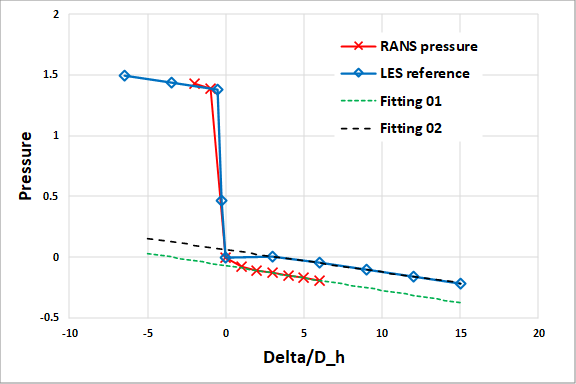
\includegraphics[width=0.5\textwidth]{./figures/Results_pressure_loss.png}
\caption{Comparison of the pressure drop from LES reference and the RANS test with momentum sources at Re = 10,000. }
\label{fig:presloss}
\end{figure}

The similar calibration has also been carried out for all other Reynolds numbers identified in this investigation, and good agreements are obtained between the LES reference results and the RANS results with momentum sources. More details about the model application in the full core models will be presented in the following sections.

%%---------------------------------------------------------------------------%%
\section{Description of the numerical models}
\label{sec:model}

In this section we discuss the numerical setup related to the full core simulations performed.
The full core configuration used is the one provided in a previous publication. A schematic of the core is provided in Figure~\ref{fig:core} featuring 37 identical assemblies. The assembly design is identical to what discussed in previous publications with a 17x17 configuration
\cite{merzari2020wall}.

\begin{figure}[!ht]
\centering
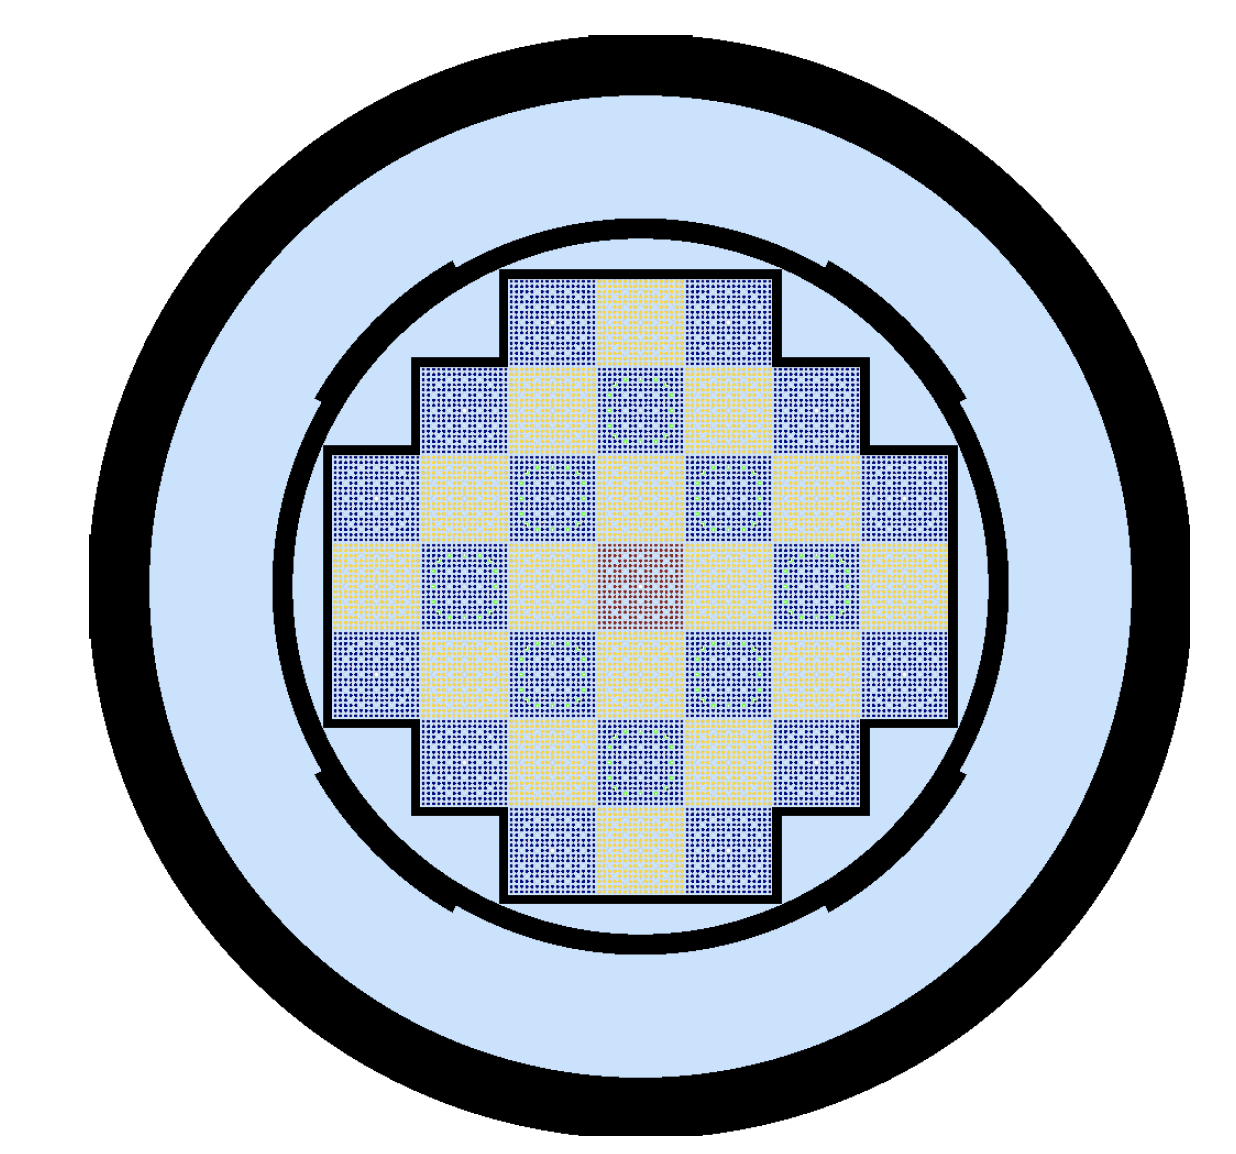
\includegraphics[width=0.5\textwidth]{./figures/core_slice.png}
\caption{Core slice showing the geometry.}
\label{fig:core}
\end{figure}

All calculations performed as part of the full core simulation campaign use the same base 2D fluid mesh, which is then extruded in the axial direction. Each fluid layer contains over a million elements. The conjugate heat transfer case examined has also mesh for the cladding, the gap and the rods, and each CHT layer contains over 2 million elements. The GLL points at polynomial order $N=2$ obtained from the mesh devised for the fluid portion of the domain is shown in Figure~\ref{fig:mesh1}.

\begin{figure}[!ht]
\centering
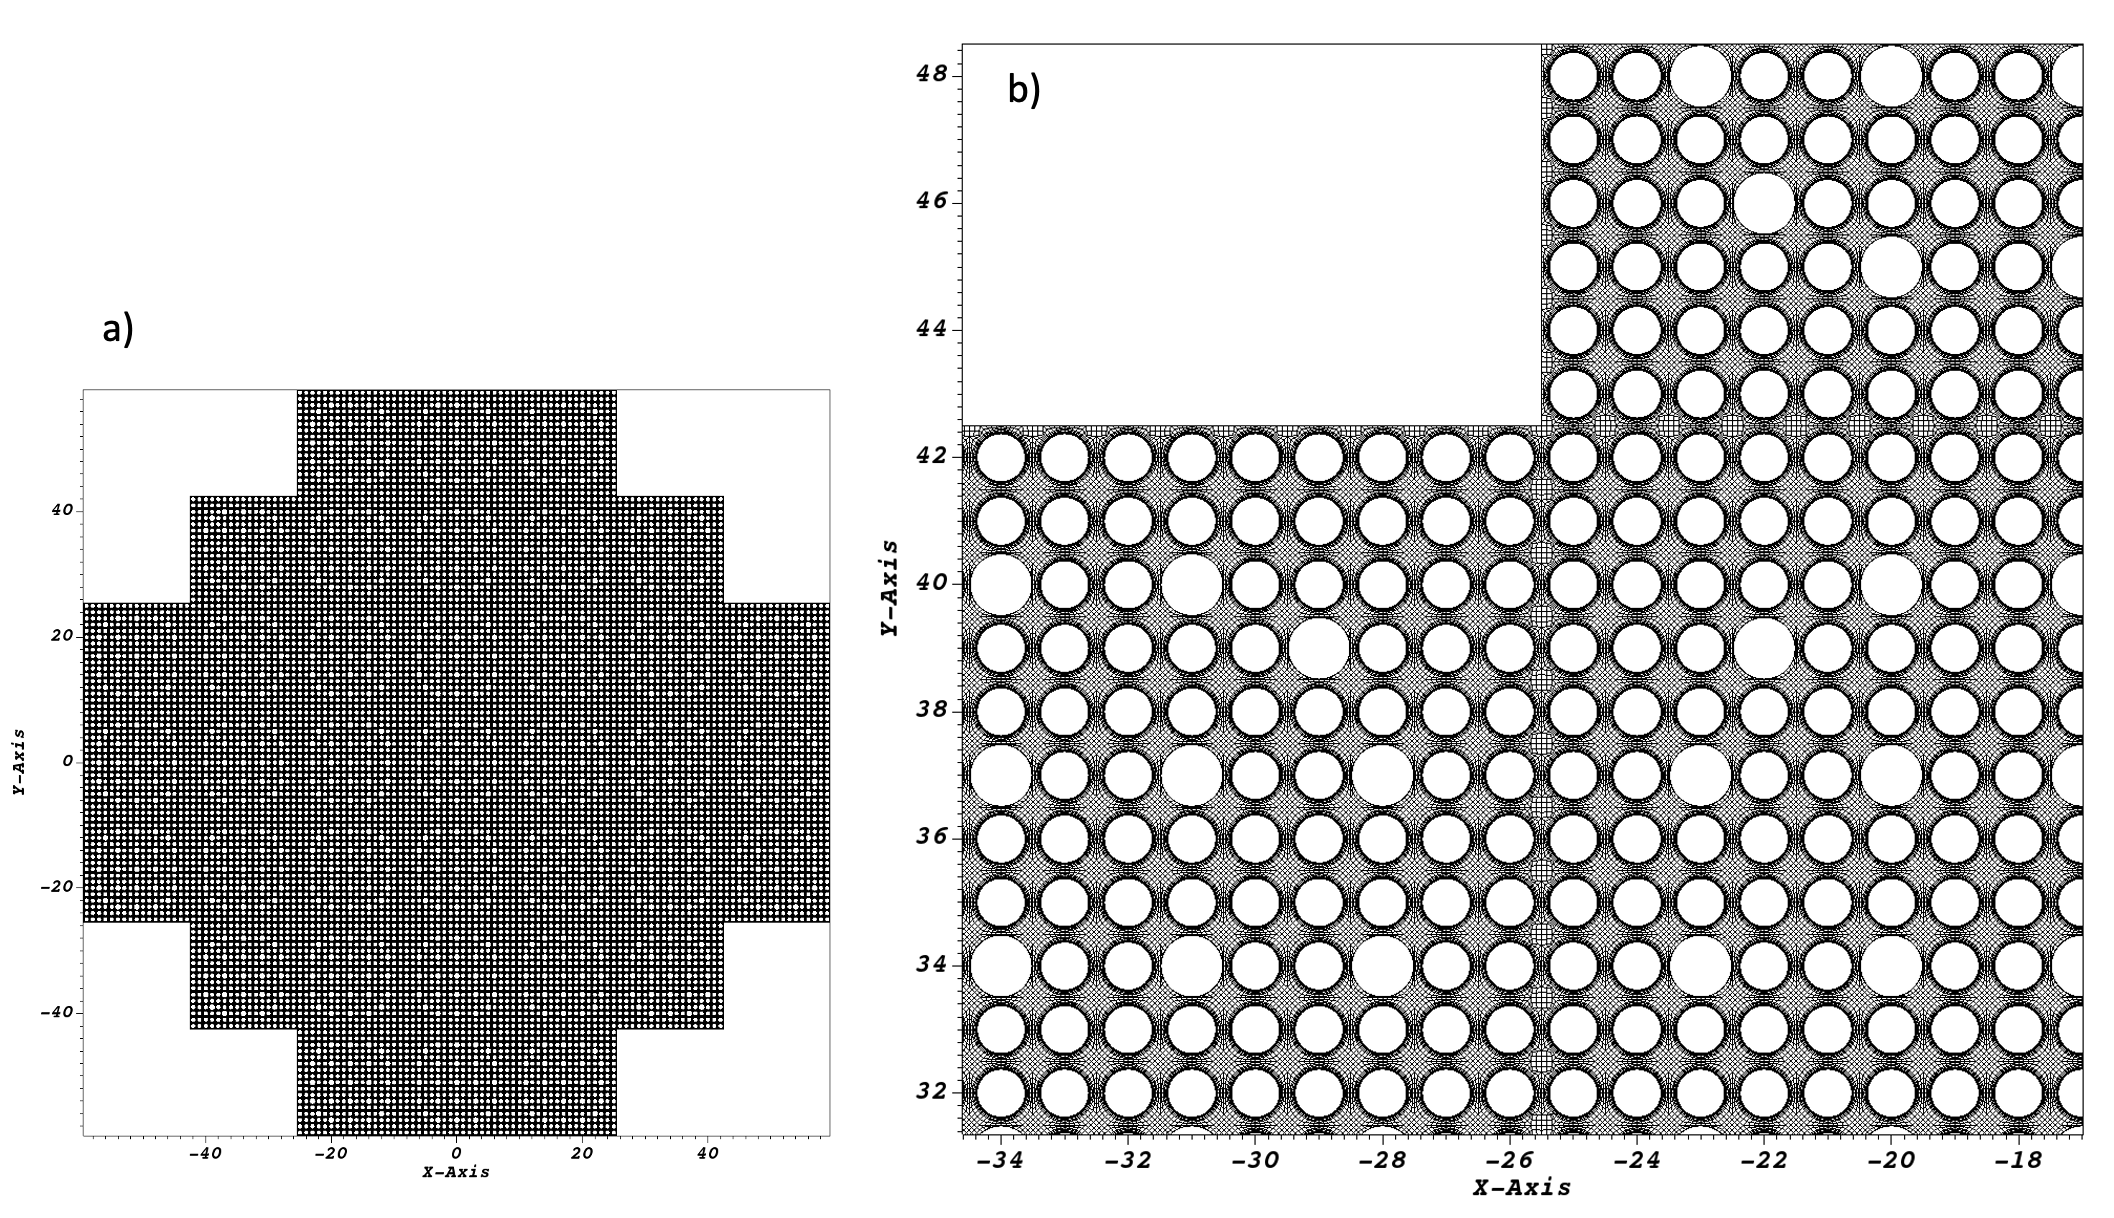
\includegraphics[width=0.99\textwidth]{./figures/full_core_mesh.png}
\caption{Mesh for the full core simulations. 2D section at low polynomial order. a) full core, b) detail.}
\label{fig:mesh1}
\end{figure}

Table~\ref{tab:full core} includes data for six representative cases, as part of this simulation campaign. Cases III and V represent full height core simulations with and without momentum sources performed with RANS. Case VI represent an initial simulation performed with Conjugate heat transfer. Most cases involve inlet/outlet boundary conditions. Case I is the case used the updated FOM calculation for ExaSMR.

\begin{table} \centering \small
% \resizebox{0.48\textwidth}{!}{
 \begin{tabular}{ccccc} \hline \hline
  Case & Boundary conditions & Model & Number of Layers $n$ & Grid points \\ \hline
   I & inlet/outlet & Large Eddy Simulation & 174 & $59.8 \cdot 10^{9}$ \\
   II & periodic slice & RANS & 3 & $1.1 \cdot 10^{9}$ \\
   III & inlet/outlet & RANS & 100 & $35.8 \cdot 10^{9}$ \\
   IV & inlet/outlet & Momentum sources, RANS & 15 & $5.2 \cdot 10^{9}$ \\
   V & inlet/outlet & Momentum sources, RANS & 100 & $35.8 \cdot 10^{9}$ \\
   VI & inlet/outlet & Conjugate Heat Transfer & 50 & $38.8 \cdot 10^{9}$ \\
   \hline \hline
\end{tabular}
 \caption{Full core cases performed: description of setup}
 \label{tab:full core}
\end{table}

%%---------------------------------------------------------------------------%%
\section{Results}
\label{sec:results}

In this section we describe briefly some selected results related to the flow in the full core and the cases described in Section~\ref{sec:model}.

\subsection{Full core simulations and FOM update}
\label{sec:results1}

The first we examine is Case I which is the largest at $59.8 10^{9}$ unique grid points. This is the case used to determine updated FOMs for the CFD component of ExaSMR. The layer size and time step $dt=3 \cdot 10^{-4}$ are consistent with previous calculation performed.  This simulation campaign corresponds effectively to a strong scaling study for the full core mesh ranging from 40\% to 100\% of Summit.

Details of the strong scaling study are provided in Figure~\ref{fig:strong} illustrating the time per time step as the simulation progresses and the overall wall time. An average time per time-step is determined as an average between 100 and 200 time steps. We note that for the previous FOM calculation this number was determined between 50 and 100 steps. However this difference is likely has a  minimal effect on the overall FOM, as the time per time-step does not change in average significantly after 50 steps. We note that the red line in Figure~\ref{fig:strong}  represents a separate strong scaling study where the 17x17 mesh is simply extruded in the streamwise direction.

\begin{figure}[!ht]
\centering
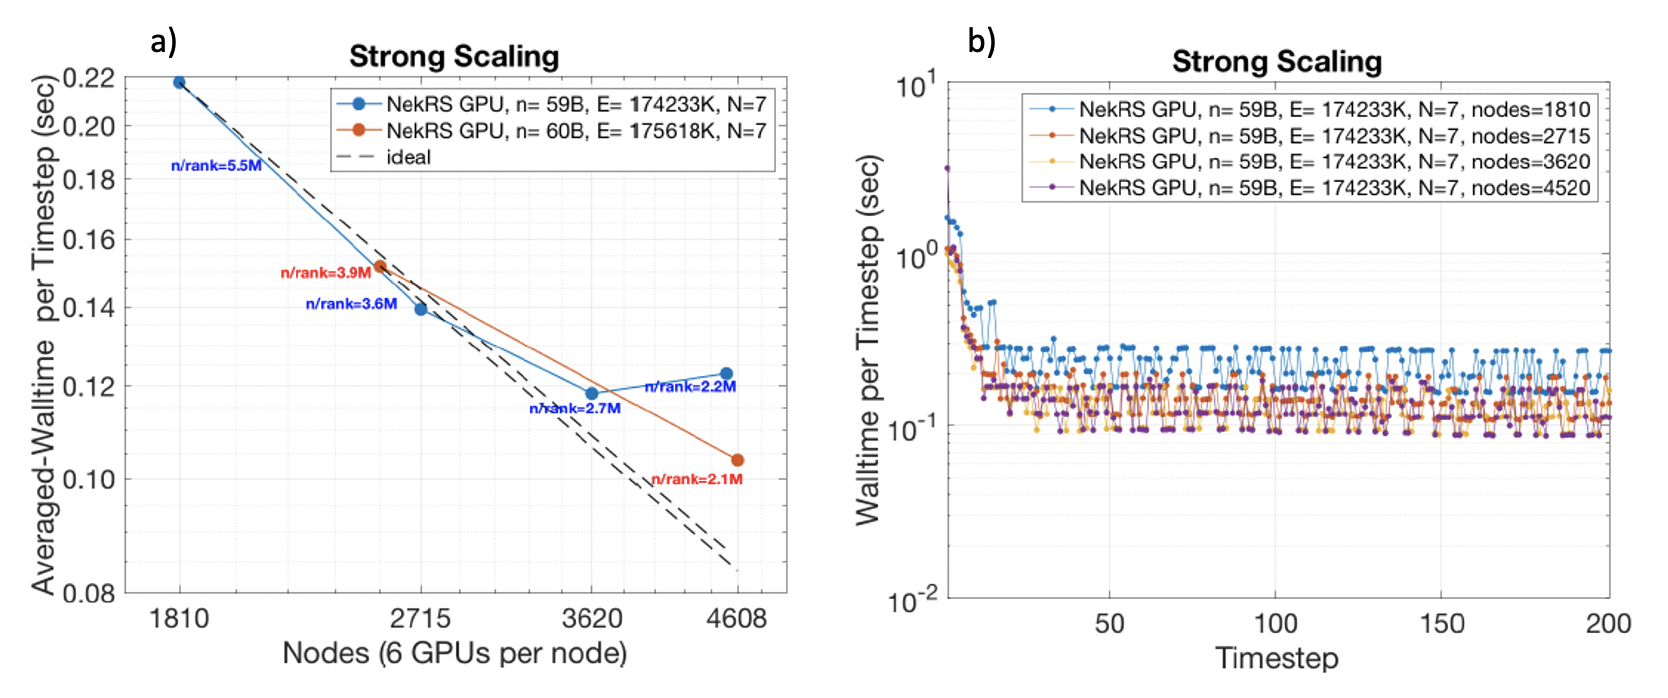
\includegraphics[width=0.99\textwidth]{./figures/full_core_strong.png}
\caption{Full core strong scaling study. a) average wall time per step. b) time per time step as simulation progresses. }
\label{fig:strong}
\end{figure}

The data collected has been used to generated updated FOM measurements in Table~\ref{tab:FOM}. This table includes both the measured FOM and the projected FOM to full machine for each of the cases. The cases with lower number of nodes should be considered a more accurate representation of full core projections for larger cases. The higher node counts are clearly below the strong scaling limit and likely do not have a sufficient number of elements and dofs per GPU.

We note that the FOM measured is significantly higher than the previous projected measurement on Summit: $1.44 \cdot 10^{11}$ dofs/s. The value reported show a 4.9x increase in projected values. We also note that the performance now is orders of magnitude higher than the FOM measured on Titan in 2018.

% Full core: n= 5.9762e+10 = E*N^3,          Previous 30M:  before (dofs/s)= 1.44506e+11
% node  rank   E                E/gpu  N  nstep  dt           cfl       t_step     avg_t_step       n/t_step     n/avg_t_step          1.44506e+11/(n/t_step)     1.44506e+11/(n/avg_t_step)
%4525  27150  174233000  6417   7  100    3.0e-04  0.58    9.34e-02   1.22e-01      6.3985e+11   4.8985e+11           4.4278e+00                      3.3898e+00
%4608  27648  174233000  6301   7  100    3.0e-04  0.58    9.01e-02   1.21e-01      6.6328e+11   4.9390e+11

 \begin{table} \centering \small
  % \resizebox{0.48\textwidth}{!}{
   \begin{tabular}{cccccc} \hline \hline
    Nodes & $E$/GPU & Fraction of machine & Average Time per step [s] & FOM (dofs/s) & Projected FOM (dofs/s) \\ \hline
    1810 & 	16043 & 0.393 &	0.2175  & $2.75 \cdot 10^{11}$ & $7.00 \cdot 10^{11}$ \\
    2715 &	10695 & 0.589 &	0.1395  & $4.29 \cdot 10^{11}$ & $7.28 \cdot 10^{11}$ \\
    3620 &	8021 & 0.786 &	0.1182  & $5.06 \cdot 10^{11}$ & $6.44 \cdot 10^{11}$ \\
    4525 &	6417 & 0.981 &	0.1229  & $4.87 \cdot 10^{11}$ & $4.95 \cdot 10^{11}$ \\
    4608 &	6301 & 1.000 &	0.121   & $4.94 \cdot 10^{11}$ & $4.94 \cdot 10^{11}$ \\
     \hline \hline
  \end{tabular}
   \caption{FOM measurement based on full core mesh. $E=174233000$, $N=7$.}
   \label{tab:FOM}
  \end{table}

\subsection{RANS full core simulations}
\label{sec:results2}

Several RANS simulations with the $k-\tau$ model have been performed as part of this campaign (see Table~\ref{tab:full core}). The numerical setup for the all the runs is consistent with the simulations discussed in Section~\ref{sec:nrs1}, which featured a verification study against Nek5000. In particular, crucial is the setup of the inlet boundary conditions. The cases have been run for a range of Reynolds numbers ($Re=10,000$ to $Re=60,0000$). The mesh was in fact  designed to support RANS simulations with $y+<1.0$ up to $Re=60,0000$.

Results from the periodic case (Case II) and the full height core case (Case III) yield identical results, at sufficient distance from the inlet. Sample results are provided in Figure~\ref{fig:vz} and Figure~\ref{fig:tke}. They illustrate a full core view and a detail for both the stream-wise velocity and the turbulent kinetic energy.  Both results are consistent with expectations and demonstrate inhomogeneous behavior near the thimbles and the boundaries of the core.

\begin{figure}[!ht]
\centering
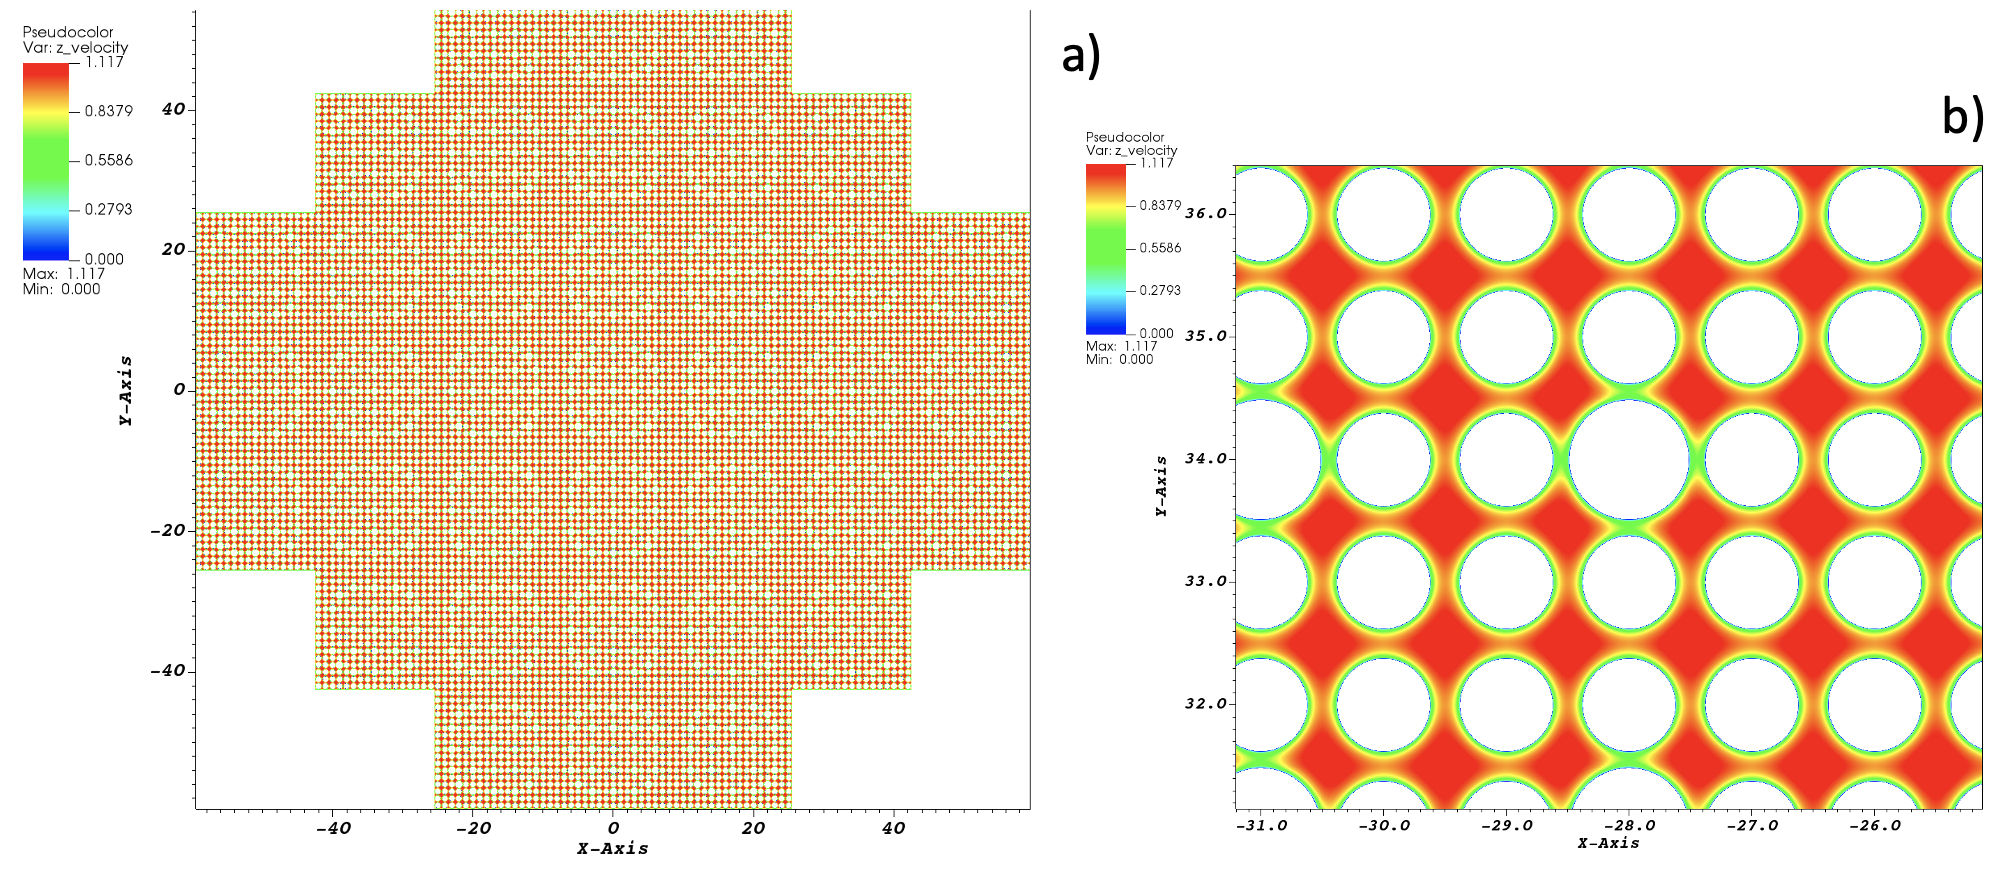
\includegraphics[width=0.99\textwidth]{./figures/periodic_vz.png}
\caption{Streamwise cross section of the velocity field ($Re=20,000$) in the fully developed region. Color plot of the streamwise velocity normalized by the bulk velocity. a) full core view. b) detail.}
\label{fig:vz}
\end{figure}

\begin{figure}[!ht]
\centering
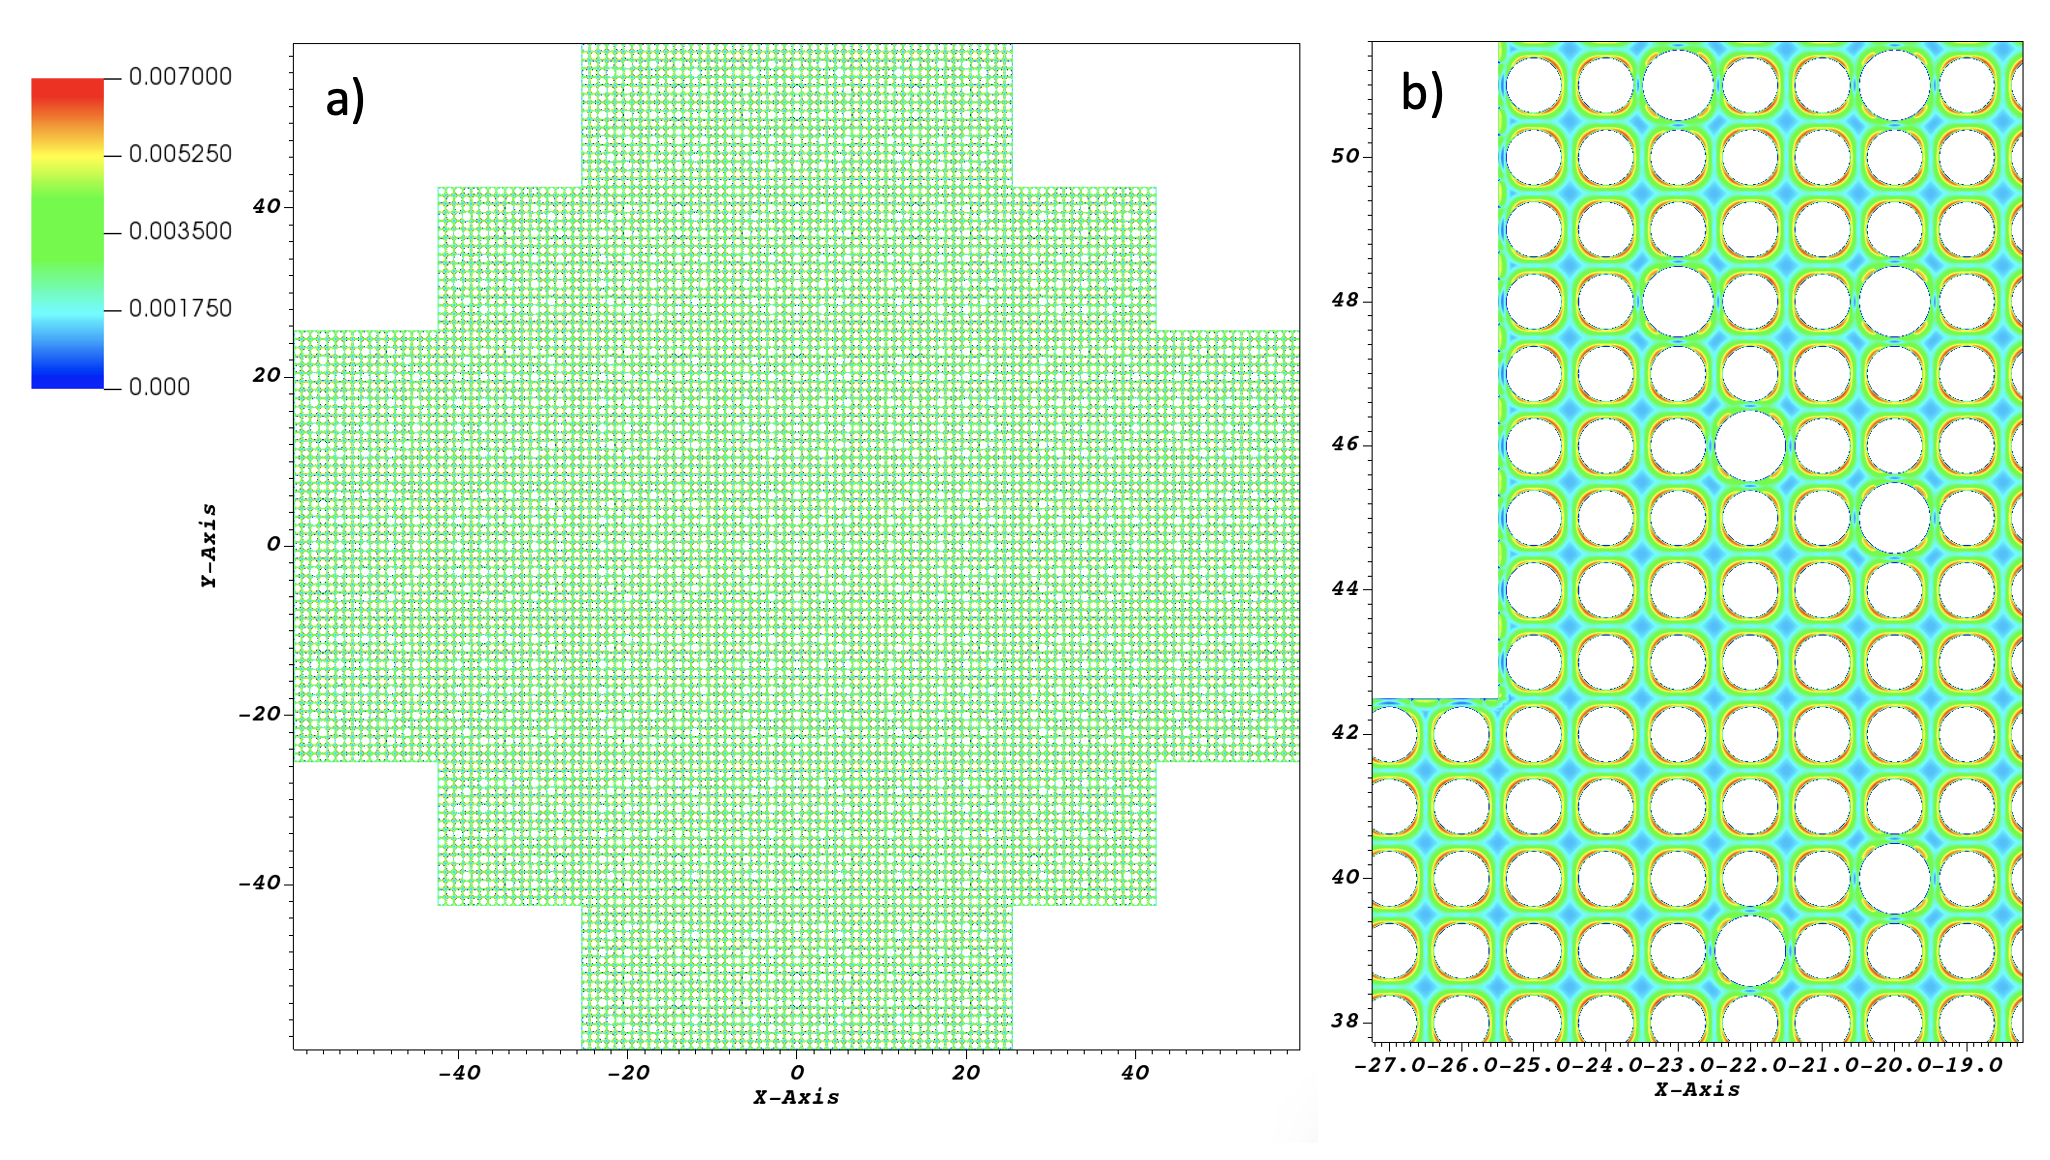
\includegraphics[width=0.99\textwidth]{./figures/periodic_tke.png}
\caption{Streamwise cross section of the velocity field ($Re=20,000$) in the fully developed region. Color plot of the turbulent kinetic energy. a) full core view. b) detail. }
\label{fig:tke}
\end{figure}

\subsection{RANS full core simulations with momentum sources}
\label{sec:results3}

The next step from Section~\ref{sec:results2} is to add appropriate momentum sources as developed through the procedure discussed in Section~\ref{sec:msm}. This was accomplished in cases IV and V.

 The momentum source was implemented in NekRS using the same approach developed in Nek5000 as leveraging as much as possible the same routines. In addition when extending to the full core, an appropriate interface was built to map the forces to the correct locations in the core based on a single assembly layout. An example of the layout of the forces is shown on a cross section in Figure~\ref{fig:msm}:
\begin{itemize}
    \item We assume every assembly has the same pattern;
    \item We choose to not place any force on the edge channels of each assembly;
    \item We simply repeat a simple 2x2 pattern in the interior of the assembly;
    \item We leave identical forces around the thimble, or none at all;
    \item We assume 5 grids axially.
\end{itemize}
We note that there is no particular restriction here and the choices were arbitrary to simplify the problem. The methodology allows to customize the forces as needed and have different patterns in different assemblies and at different heights.

We now show was sample results of the flow field in the full core. We pay particular attention to the cross flows. Figure~\ref{fig:msm1} shows the cross flows directly past the first grid span.

\begin{figure}[!ht]
\centering
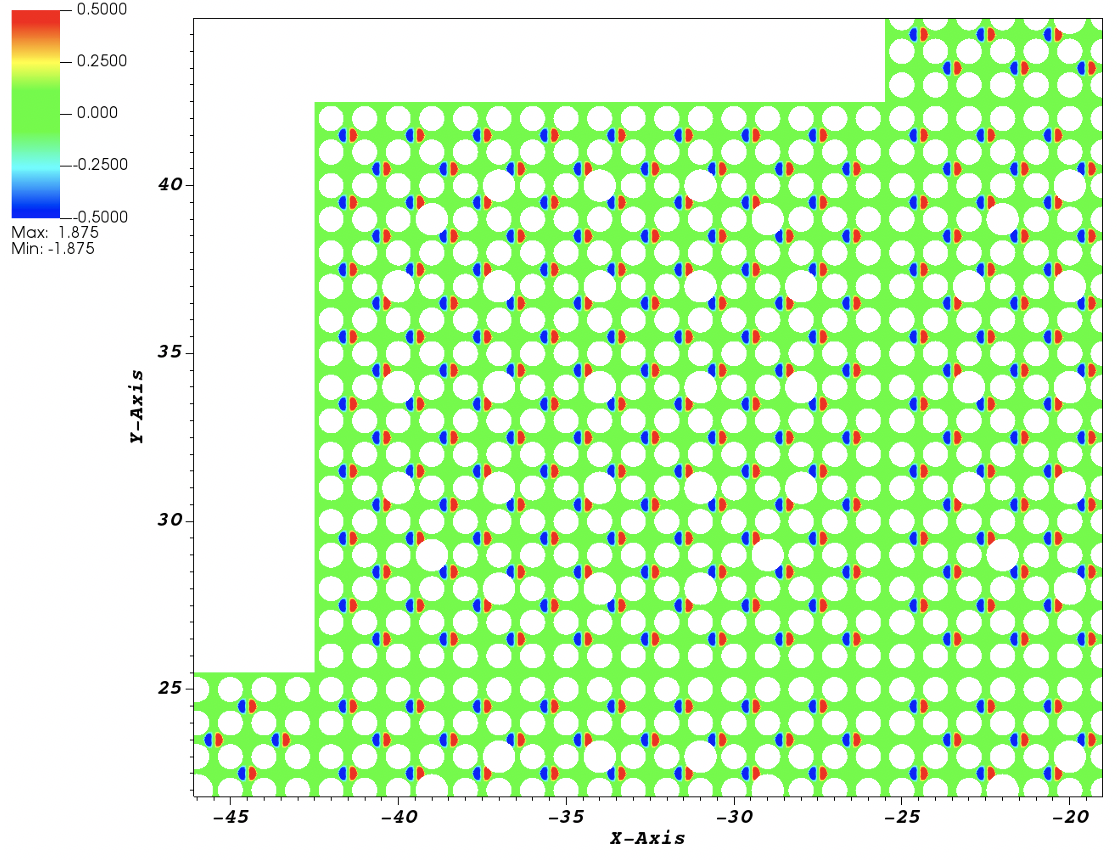
\includegraphics[width=0.99\textwidth]{./figures/1span_msm.png}
\caption{Detail of forces in full core simulation. Force in direction $y$. }
\label{fig:msm}
\end{figure}

\begin{figure}[!ht]
\centering
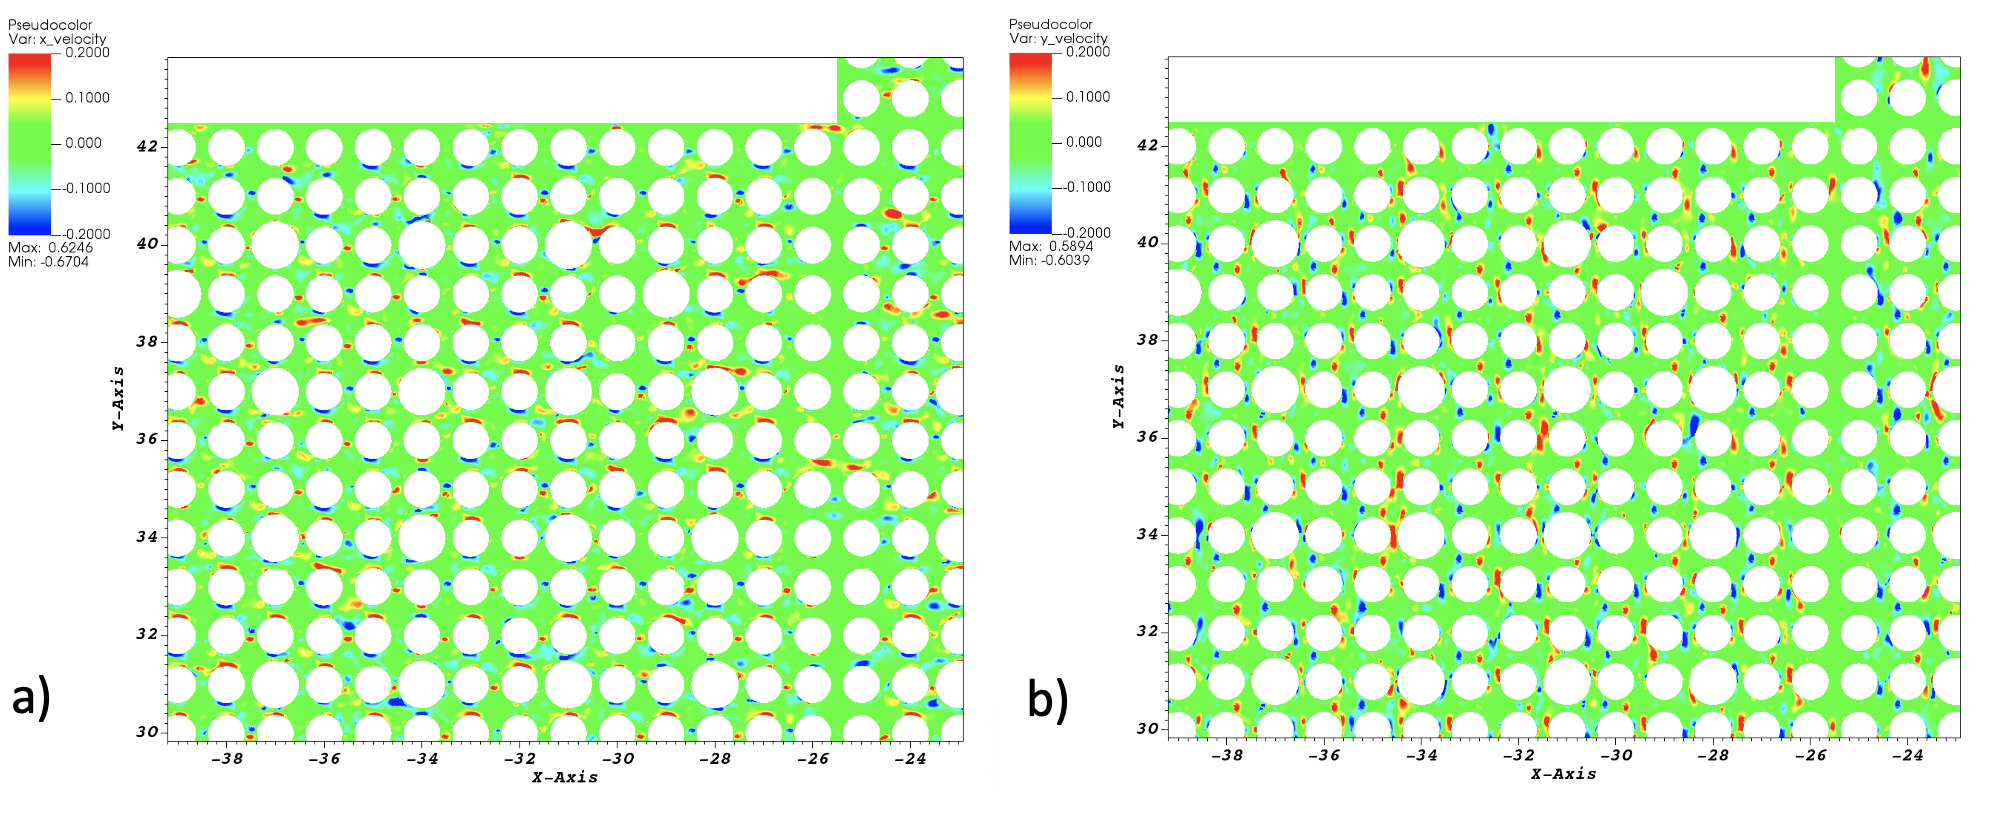
\includegraphics[width=0.99\textwidth]{./figures/1span_msm_v1.png}
\caption{Details of cross flow in full core after the spacer grid. a) Velocity in direction $x$. b) Velocity in direction $y$. }
\label{fig:msm1}
\end{figure}

\subsection{Conjugate heat transfer}
\label{sec:results4}

In addition to the full core cases demonstrated above, a quarter-height case (Case VI) was also performed for demonstration purposes of a conjugate heat transfer model representing each pin in the core. The mesh is consistent with previous 17x17 assembly calculations performed for coupled analysis with ENRICO. The gap and cladding are modeled explicitly as well as the fuel. A very preliminary result is shown in Figure~\ref{fig:cht}, for the beginning of transient.

\begin{figure}[!ht]
\centering
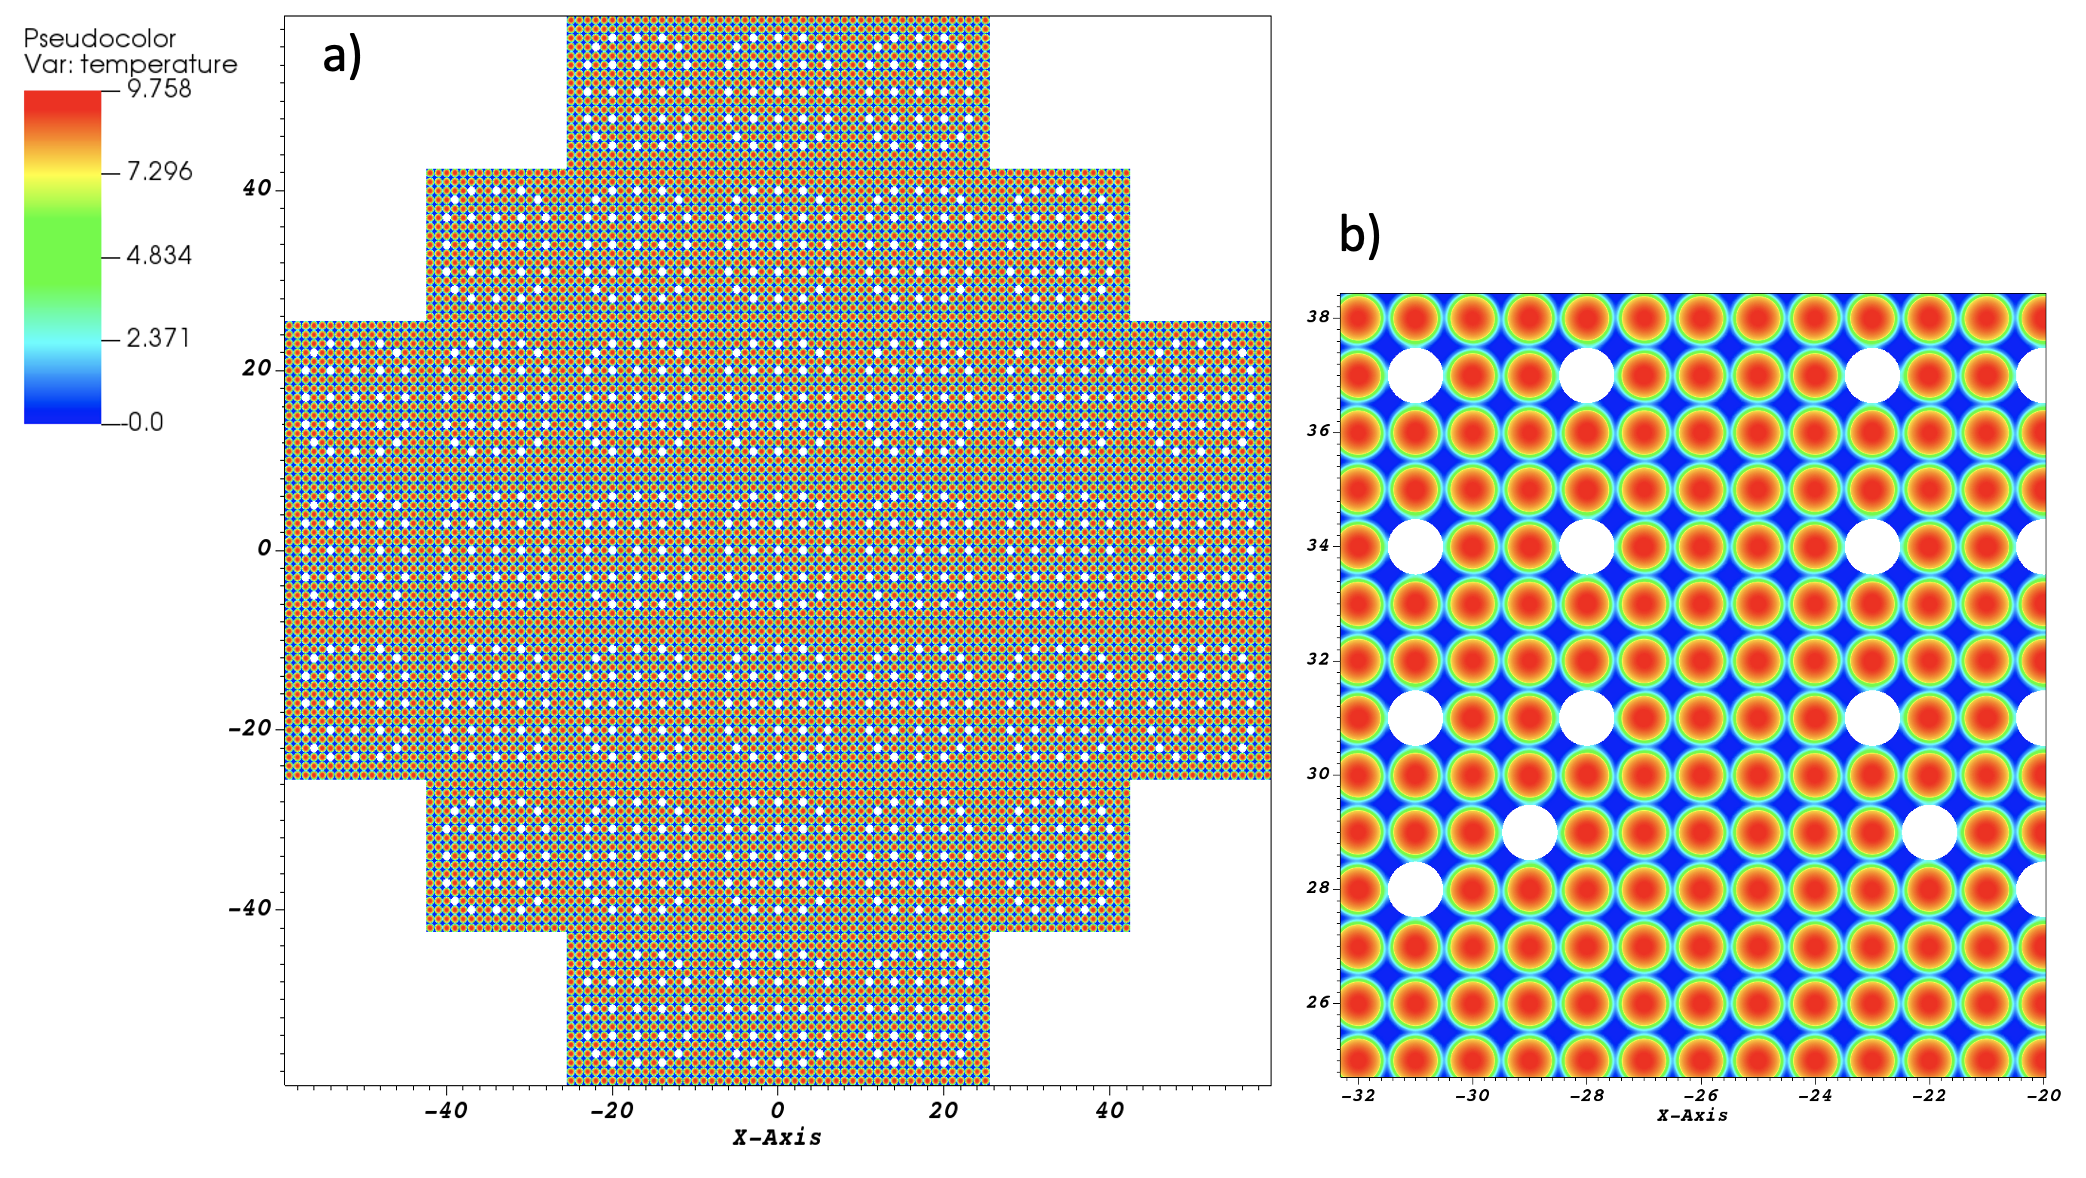
\includegraphics[width=0.99\textwidth]{./figures/quarter_cht.png}
\caption{Conjugate heat transfer results for full core, full view and detail. Temperature in arbitrary units.}
\label{fig:cht}
\end{figure}

%%---------------------------------------------------------------------------%%
\section{Conclusions and Future Work}
\label{sec:conc}

In this report we discussed a series of simulations performed with NekRS for an SMR full core simulation. We reiterate that \textit{this milestone provides the first full-core pin resolved simulations ever performed to our knowledge}. The capability developed is significant advancement for the field of applied CFD in nuclear engineering.

The simulations perfortmed covered both Large Eddy Simulation and Reynolds Averaged Navier Stokes. The Reynolds Averaged Navier-Stokes simulations include modeling of the spacer grid effects, a key aspect of the flow in PWR cores, through momentum sources. The momentum sources have been developed and calibrated using Large Eddy Simulation in a 5x5 assembly with the spacers and the vanes explicitly modeled. We note that there is considerable literature already on the validation of Nek5000 for spacer grids \cite{BUSCO2019144} \cite{yuan2020spectral}. This report presents the first set of simulations in which a momentum sources approach has been applied to a full core.

The Large Eddy Simulation results for the full core have been used to define a new FOM for ExaSMR. The obtained results mark a significant improvement compared to the previous value on Summit (4.8x increase). They also represent the first full machine measurement with NekRS.  The performance is now two orders of magnitude higher than on Titan (with the OpenACC version of Nek5000). We note that this corresponds to broad improvements to the code and it is not an isolated case. Similar speed-ups have been reported for a broad range of production runs.

In the future we will perform full core, full height conjugate heat transfer calculations and work toward performing full core coupled calculations with Monte Carlo. This is currently limited by integer overflow in Nek5000 and NekRS (the maximum number of elements is $E=180,000,000$). We are working to remove this limitation. We will also implement a zonal hybrid approach  for the full core. In this approach the core is modeled with URANS and momentum source while in one of the assemblies the spacer grids are modeled explicitly and turbulence is modeled with LES.


%%---------------------------------------------------------------------------%%
\section*{Acknowledgments}

This research was supported by the Exascale Computing Project (ECP), Project
Number: 17-SC-20-SC, a collaborative effort of two DOE organizations---the
Office of Science and the National Nuclear Security Administration---responsible
for the planning and preparation of a capable exascale ecosystem---including
software, applications, hardware, advanced system engineering, and early testbed
platforms---to support the nation's exascale computing imperative. We gratefully
acknowledge the computing resources provided by the Joint Laboratory for System
Evaluation at Argonne National Laboratory. This research used resources of the
Oak Ridge Leadership Computing Facility at the Oak Ridge National Laboratory,
which is supported by the Office of Science of the U.S. Department of Energy
under Contract No. DE-AC05-00OR22725.

%%---------------------------------------------------------------------------%%
%% References

\bibliographystyle{unsrt}
\bibliography{references}

%%---------------------------------------------------------------------------%%
%% APPENDICES
%%---------------------------------------------------------------------------%%

%%---------------------------------------------------------------------------%%

\end{document}

%%---------------------------------------------------------------------------%%
% end of report.tex
%%---------------------------------------------------------------------------%%
